\documentclass[12pt]{article}
\usepackage[a4paper, portrait, margin=1cm, right=1cm]{geometry}
\usepackage{fontspec}
\usepackage[fleqn]{amsmath}
\usepackage{setspace}
\usepackage{graphicx}

\graphicspath{./graphics/}
\setmainfont[Ligatures=TeX]{Linux Libertine}

\title{Информационные технологии. Лекция 01. КФС. Основные свойства. БТС}
\author{Студент группы 2305 Макурин Александр}
\date{07 февраля 2023}

\begin{document}
\maketitle
\begin{sloppypar}
    \setstretch{1.8}

    \section*{Организационные вопросы}
    \subsection*{Список лабораторных (каждая даёт 10 баллов)}
    \begin{itemize}
        \item Начало работ с Gazebo
        \item Создание модели ТС (БПЛА, БТС)
        \item Автономное ТС
        \item Реализация протоколов связи
        \item Роевой интеллект на группе ТС
        \item Стратегическое планирование
    \end{itemize}
    \subsection*{Оценки}
    \begin{itemize}
        \item 95\%+ (57+ баллов) = 5
        \item 90\%+ (54+ баллов) = 4
        \item 80\%+ (48+ баллов) = 3
    \end{itemize}

    \section*{Индустрия 4.0 - замещение людей роботами}

    БТС - беспилотное транспортное средство

    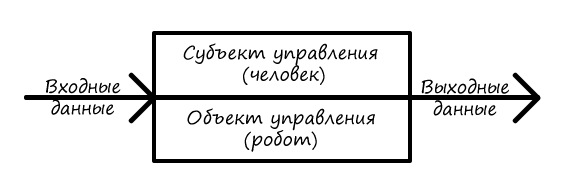
\includegraphics[width=0.5\textwidth]{graphics/СУ_ОУ.png}

    Кибер-физическая система (КФС) - система, интегрирующая способности к вычислениям,
    связи и хранению информации с мониторингом и/или управлением объектами
    физического мира и должна делать это надёжно, безопасно, эффективно и в
    реальном времени.

    АСУ ТП становятся всё менее распространёнными по причинам плохой
    расширяемости (одна система управления на множество датчиков и механизмов) и
    коррупции в научной среде.

    \section{История робототехники}
    \begin{itemize}
        \item Движущиеся статуи (I век до нашей эры)
        \item Механические устройства (Леонардо да Винчи)
        \item Автоматоны (Пьер Жаке-Дро)
        \item Разностная машина (Чарльз Бэббидж)
        \item Boilerplate (Арчи Кемпион)
    \end{itemize}

    \section{Промышленные роботы}
    \begin{itemize}
        \item Манипуляторы
        \item Johns Hopkins Beast (1960) — робот, решающий главную задачу всех
              роботов (найти поесть) Он умел искать розетки, от которых
              подзаряжался, в белой комнате с чёрными розетками.
              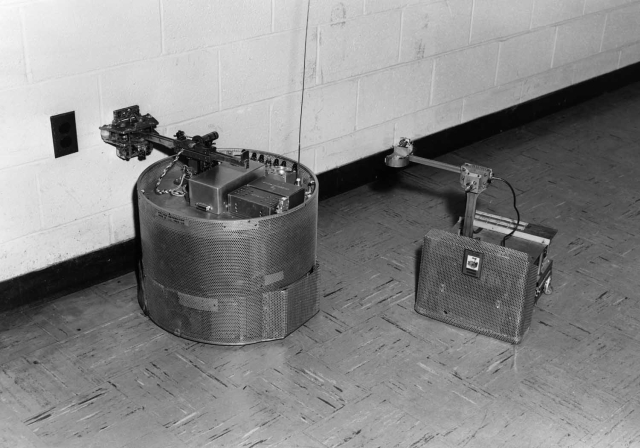
\includegraphics[width=0.7\textwidth]{graphics/johns_beast.jpg}
        \item Shakey (1970)
        \item Луноход
        \item Марсоход
    \end{itemize}

    Задача грузчика — как двум роботам перенести пианино. Не решённая задача.
    Для решения требуется найти алгоритм нахождения баланса между двумя роботами
    и пианино.

    Робо-рука для сбора помидоров — требует контроля силы сжатия/удержания
    помидора.

    \section{Тенденции развития}
    \begin{itemize}
        \item Разработка стандартов
        \item Уменьшение размеров
        \item Удешевление стоимости комплектующих
        \item Развитие систем управления:
              \begin{itemize}
                  \item ИИ
                  \item Стайное управление
                  \item Функционирование в условиях неопределённости
              \end{itemize}
    \end{itemize}
    \subsection*{Три уровня планирования:}
    \begin{itemize}
        \item Оперативный — копипаст со Stack Overflow - решение текущей задачи
        \item Тактический — Junior $\rightarrow$ Middle $\rightarrow$ Senior
        \item Стратегический — главная цель, на которую направлены задачи всех
              остальных уровней, например, увеличение прибыли
    \end{itemize}

    Разработка стандартов — Разработка правил, по которым можно было бы создать
    ИИ, который точно не сойдёт с ума — не восстанет против человека, будет
    выполнять свою задачу.

    \setstretch{1}
    \[
        \begin{array}{ccccc}
            E              & = & E^{\textit{inf}}               & \cup & E^{phy}                    \\
            \uparrow       &   & \uparrow                       &      & \uparrow                   \\
            \text{система} &   & \text{информационные элементы} &      & \text{физические элементы}
        \end{array}
    \]
    \begin{center}
        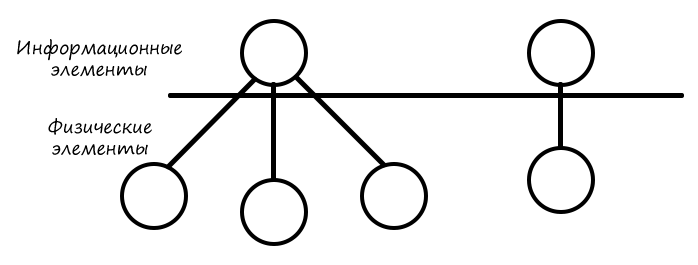
\includegraphics[width=0.5\textwidth]{graphics/Информационные_и_физические_элементы.png}
    \end{center}
    \[
        \begin{array}{ccccc}
            S_E                      & = & f( & E,             & U)                         \\
            \uparrow                 &   &    & \uparrow       & \uparrow                   \\
            \text{состояние системы} &   &    & \text{система} & \text{входные воздействия}
        \end{array}
    \]
    \setstretch{1.8}

    \subsection*{Система}

    \begin{center}
        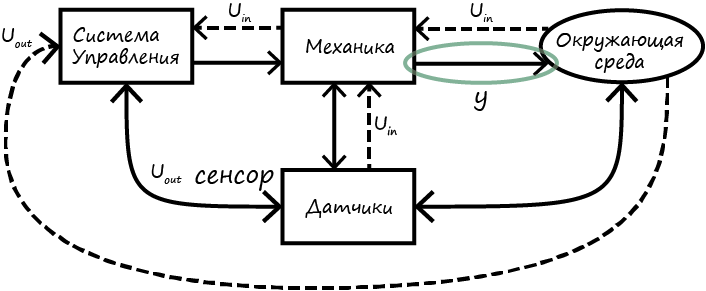
\includegraphics[width=0.7\textwidth]{graphics/Система.png}
    \end{center}

    \[
        U = U_{out} \cup U_{in}
    \]

    $y$ — выходные параметры

    $|y| = |U|$. Или, другими словами, размерность $y$ = размерность $U$

\end{sloppypar}
\end{document}